\setcounter{section}{4}
\section{Preparation Activity 5 - REs}
{
\renewcommand{\thesubsubsection}{\thesubsection\alph{subsubsection}}
\subsection{Exercise 1}
\begin{equation*}
	(a+b+c)^\ast ((abc(\varepsilon+(a+b+c)^\ast c)ba)+(cba(\varepsilon + (a+b+c)^\ast a)bc))(a+b+c)^\ast
\end{equation*}
\subsection{Exercise 2}
\subsubsection{Item a}
\begin{center} 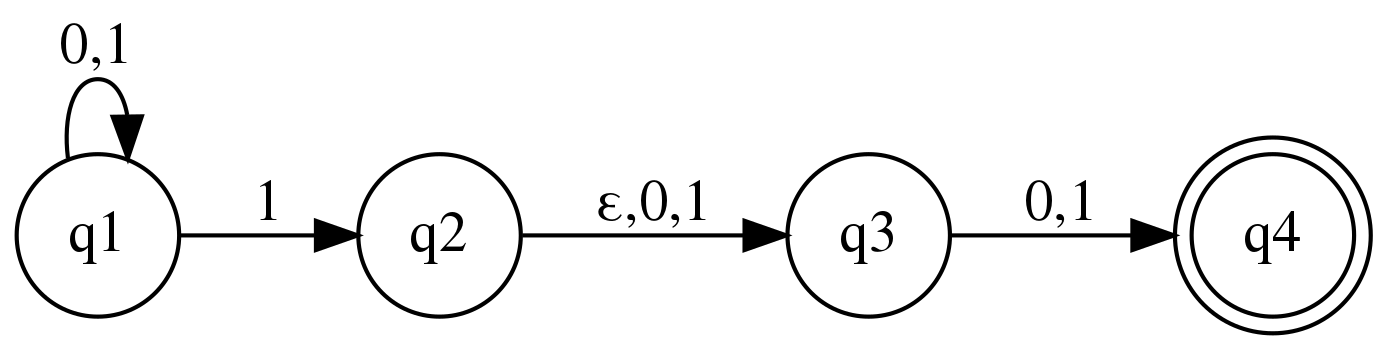
\includegraphics[scale=0.12]{PA05_2a_1} \end{center}
\begin{center} 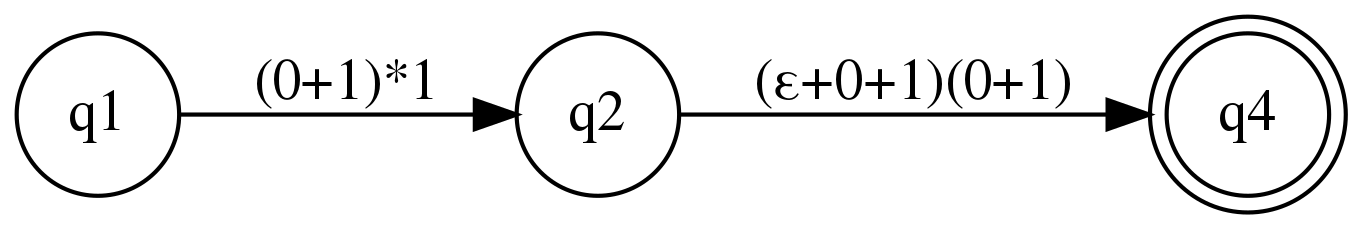
\includegraphics[scale=0.12]{PA05_2a_2} \end{center}
\begin{center} 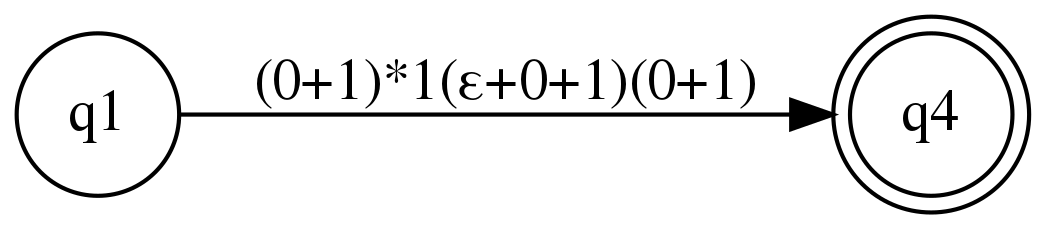
\includegraphics[scale=0.12]{PA05_2a_3} \end{center}
\begin{equation*}
	(0+1)^\ast 1(\varepsilon+0+1)(0+1)
\end{equation*}
\textcolor{red}{Incomplete}
}